\documentclass[border=10pt]{standalone}
\usepackage{pgfplots}
\pgfplotsset{compat=1.18}
\usepgfplotslibrary{colormaps}

\begin{document}

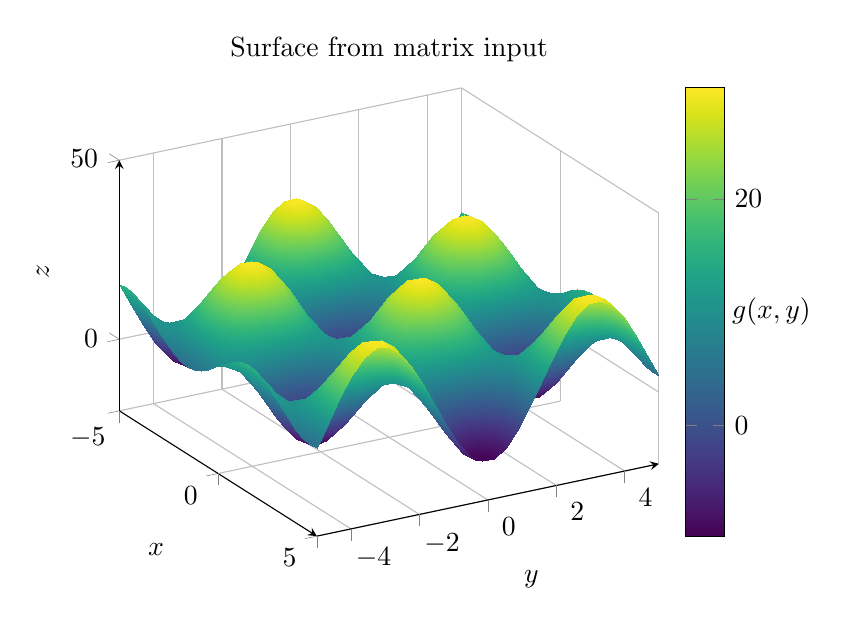
\begin{tikzpicture}
    \begin{axis}[
        title={Surface from matrix input},
        xlabel=$x$, ylabel=$y$, zlabel=$z$,
        view={60}{30},
        colormap/viridis,
        colorbar,
        colorbar style={
            ylabel={$g(x,y)$},
            ytick={-20,0,20,40},
            yticklabels={-20,0,20,40},
            width=5mm,
            ylabel style={rotate=-90, at={(ticklabel cs:0.5)}, anchor=center},
        },
        xmin=-5, xmax=5,
        ymin=-5, ymax=5,
        zmin=-20, zmax=50,
        grid=major,
        samples=30,
        domain=-5:5,
        y domain=-5:5,
        shader=interp,
        axis lines=left,
        tick align=outside,
        enlargelimits=false,
    ]
    \addplot3[surf] {sin(deg(x)) * cos(deg(y)) * 20 + 10};
    \end{axis}
\end{tikzpicture}

\end{document}